\documentclass{article}
\usepackage{amsmath}
\usepackage{mathtools}
\usepackage{txfonts}
\usepackage[margin=0.5in]{geometry}
\usepackage{graphicx}
\usepackage{float}
\graphicspath{ {images/} }


\setlength{\parskip}{\baselineskip}%
\setlength{\parindent}{0pt}%

\title{A regression model for predicting rail transit ridership at the station level}
\author{Daniel Hartig}
\date{\vspace{-5ex}}


\begin{document}
\maketitle

\section{Introduction}

The United States is undergoing a rail boom. Since 2010, new light rail lines have opened in Dallas, Los Angeles, Salt Lake City, Denver, Minneapolis, Houston, Seattle and more.  A new heavy rail line opened in Washington DC, and a commuter rail system in Orlando. As transit expands in cities in the United States, there is an opportunity to validate predictive rail ridership models. 

A survey of transit agencies\cite{Boyle2006} conducted by the Transit Cooperative Research Program showed that relatively few agencies are using quantitative models when forecasting ridership for new lines, extensions or stations under consideration for funding. Of the 35 agencies that responded to the survey, 29 use professional judgment and 28 use rules of thumb among one or more techniques used to generate ridership forecasts. Another method used by 22 agencies is service elasticity; a set of general transit demand response curves for changing transportation options, published by the Transportation Reserach Board \cite{tcrp95}. 

For quantitative methods, the most commonly used technique--by 18 of 35 surveyed agencies--is the four-step travel demand model\cite{McNally2008}, introduced by Mannheim and Florian\cite{Mannheim1979, Florian1988}. The Mannheim-Florian model's four steps are trip generation, trip distribution, mode choice and route choice. In the trip generation phase, trip endpoints are created with as production and attraction ends. In the trip distribution step, these endpoints are paired up to generate trips; for example a residence with a a job, or hotel with a tourist attraction. In the mode choice step, trips are assigned to various transportation modes, such as personal vehicle, bus, or walking. Finally, in the route choice step, a route using that mode of transportation is chosen.

An implementation of the Mannheim-Florian model can be seen in the Seattle's Sound Transit Ridership Forecasting Methodology Report\cite{ST3_2015, ST3_add}. The Sound Transit 3 (ST3) was a ballot measure that passed in 2016 for a \$54 billion expansion of the local light rail system involving 100 km of new tracks and 37 new stations. The ridership forecasting methodology report explained how the project's official ridership projections were developed. The regional area is divided into 785 Alternatives Analysis Zones and for each of these zones transit surveys and recorded ridership on local bus routes were used to complete the trip generation and trip distribution steps. The mode choice and route choice is done using an incremental logit model to predict changes in transit mode based on changes in transit mode availability.

Only seven of the 35 surveyed agencies used regression models among the methods to predict future transit ridership. This thesis proposes a regression-based model based on data from the United States Census Bureau at the zip code level. The model will be trained on the zip code characteristics and ridership data from existing light and heavy rail transit systems and used to predict ridership on other rail transit systems.  

The Mannheim-Florian four step model fundamentally depends on already existing transit information. For example, the starting point of a four step analysis for a new light rail line would be an existing bus line that runs a similar, hopefully identical, path. The advantage of a regression model is that it creates a new estimate from different sources. Even if a regression model's accuracy is not superior to that of a four step model used on the same transit network, the regression model is still valuable because it produces a second, independent quantitative estimate. This estimate can be used to validate or adjust any existing model. 


\section{Data and Methodology}

\subsection{Data Sources for Predictor Variables}

The zip code level data for feature generation comes from the US Census Bureau and is available at \texttt{factfinder.census.gov}. There are thousands of potential data sets available. Selection of features is guided by Kuby\cite{Kuby2004}, Taylor\cite{Taylor2008}, and Currie\cite{Currie2011}, which demonstrate the significance of factors such as employment, population, universities, poverty, airports, park and ride stations, and rental units. In Yao\cite{Yao2007}, a distinction is made between `Need Index,' a series of features that depend on the characteristics around the station and are independent of the transit network, and transit network characteristics, which do depend on the transit network. To model network characteristics for each station, the sum of each characteristic for every other station within 15 and 30 minutes transit time is included as a feature of the original station. This also provides us quantitative way to express the 'centrality' dummy variable that is provided as a flag in many models\cite{Kuby2004, Durning2015}; centrality could be proportional to the count of population or jobs within 30 minutes of a station, for example.

This model emphasizes using only feature that have 'real' units. Only a single feature (presence of a park and ride garage) is a flag. Instead of using measures of land use mix as proposed in other models\cite{Durning2015, Gutierrez2011}, or dummy variables for universities and central business districts, the equivalent information is provided naturally as counting data in the feature set. Housing types (such as large apartment buildings versus single family homes) can stand in for land use mix, number of jobs at universities or in financial jobs can file in for the equivalent dummy variable. A summary of the selected characteristics is provided in (REFERENCE TO APPENDIX).

Ridership data for agencies that publish annual ridership reports is used to validate the model. Six cities were selected for this study: Boston, Chicago, Los Angeles, Atlanta, Dallas, and Denver. Several cities were eliminated from the sample set for various reasons. The Census Bureau data set does not include government employment. While state level employment is significant in all potential cities, state employment levels are relatively constant from city to city. Federal employment varies greatly, however. Washington DC was eliminated due to the large impact of un-recorded federal employment. San Francisco and Philadelphia were eliminated because they have multiple rail systems without integrated fares. New York City was eliminated because it's subway has higher ridership than all other rail systems in the country, combined. 

The data closest to 2015 is used when possible to get an accurate relation between ridership and census data. The census data as well as Chicago, Dallas, Denver's ridership statistics are from 2015. Boston's ridership is from 2014, Los Angeles' is from 2013-2014, and Atlanta's is from 2010-2013. 



\subsection{Feature Generation}

We translate zip code level data into transit station specific data by sampling each zip code's geographic area to determine proximity to a transit station. For each zip code near the transit network, a set of random points within that zip code is generated using rejection sampling. For each of the those points, the one or more closest stations are determined. Each point is assigned to one or more station within walking distance. Counts for the characteristics of each zip code, such as population or employment, are then assigned to each station proportional to the number of points assigned to each station.

\subsubsection{Rejection Sampling of Zip Code Shapefiles}

The US Census Bureau provides TIGER/Line shapefiles of each zip code tabulation area (ZCTA) in the United States at \linebreak\texttt{https://www.census.gov/geo/maps-data/data/tiger-line.html}.  From a box drawn around the extremities of each zipcode's shape, random points are accepted if they are within the shapefile or rejected if they are outside it. Those points that are inside the shapefile are tested against author created exclusion zones. These zones are shapes within the zip code's shapefile area that are known to not have any population, employment, or other countable characteristics. The exclusion zones are mostly drawn over water areas, or large parks. Those points that are inside the exclusion zones are also rejected.

The remaining points are tested for their distance to any transit stations. The area within walking distance of a station is its catchment. A standard transit catchment distance for rail is one half mile (800 m), although Guerra\cite{Guerra2012} suggests that one half mile is more appropriate for population as a feature while one quarter mile (400 m) is better for employment. A case study\cite{ElGeneidy2014} from a 2003 Montreal transit riders origin-destination survey concluded that approximately 50\% of riders of the city's urban rail transit walk less than 500 meters to their stations, while 90\% walk less than 1000 meters. The maximum walking distance is approximately 1500 meters. Another analysis\cite{Gutierrez2011} found that a straight line distance all-or-nothing proximity function for assigning population and employment to a station optimized a subsequent regression analysis at between 600 and 900 meters. 

Given this information, we choose cutoffs of 500 meters and 1000 meters for calculating station distances. (NOTE: DO I HAVE TO EXPLAIN FURTHER WHY I CHOSE 500/1000???) Each tested point is divided between all stations within 500 meters. If there are no stations within 500 meters, then the point is divided between all stations within 1000 meters. If no stations are within 1000 meters, that point is not assigned to any station. The total sum of points and fractional points assigned to each station is divided by the total points available. The station's portion of each of the zip code's characteristic data counts is assigned to that transit station. 

\begin{figure}[H]
\begin{center}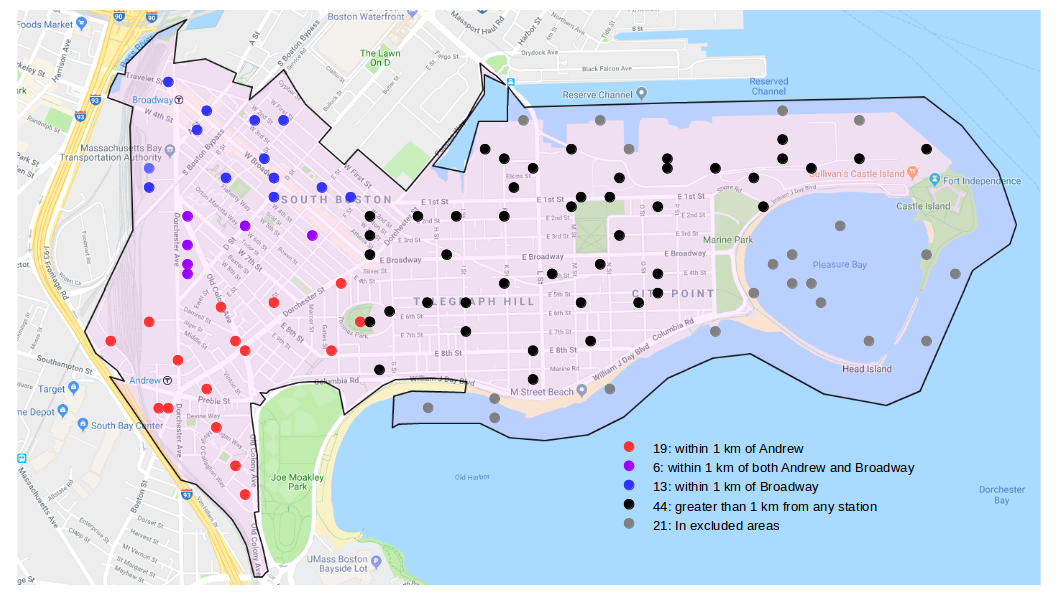
\includegraphics[scale=0.6]{geo_point_demonstration}\end{center}\caption{Illustration of nearest zip code estimation for zip code 02127.}\label{fig:f1}
\end{figure}


An example using zip code 02127, the South Boston neighborhood of Boston, illustrates the sampling method (Figure \ref{fig:f1}). 100 random points are selected within the area of the shapefile. Of these, 21 are rejected due to exclusion areas based on water area, parks and abandoned port facilities. Of the remaining 79 points, 8 are within 500 meters of Andrew station, while 6 are within 500 meters of Broadway station. Moving out to the 1000 meter radius, 11 are within 1 km of Andrew station, for a total of 19 closest to Andrew; 7 are within 1 km of Broadway station for a total of 13 closest to Broadway; and 6 are within 1 km of both. The 6 stations within 1 km of both stations are divided between the two. The total population of South Boston is 36494. Therefore, $$\frac{19 + \frac{6}{2}}{79}\cdot{36494} = 10163$$ people are assigned to Andrew station. Similarly, 7391 people are assigned to Broadway station. This calculation is performed for all countable features and all zip codes and summed total counts for each characteristic are used as a feature for each transit station. 

\subsubsection{Generation of network dependent features}

For each `Need Index' type feature generated by rejection sampling, a set of corresponding network based features are generated to represent the sum total of a certain characteristic (such as population or employment) within a given travel time of that station. The transit network is laid out as a graph, where nodes represent the transit stations and edges are weighted to the travel time between the stations, according to the website of the transit agency. At transfer points, there is a separate node for a single station on each line. The edge between these two nodes is the average wait time for transfer between the trains. 

An illustration of the calculation of travel time between Sullivan Square and South Station in Boston is provided in Figure \ref{fig:f2}. Starting at Sullivan Square on the Orange Line southbound, there are four edge traversals totaling seven minutes to get to Downtown Crossing. From there, there is a 2.5 minute wait until a Red Line (also Southbound) train arrives, and 2.5 more minutes of travel to South Station. The total travel time is thus twelve minutes. 

\begin{figure}[H]
\begin{center}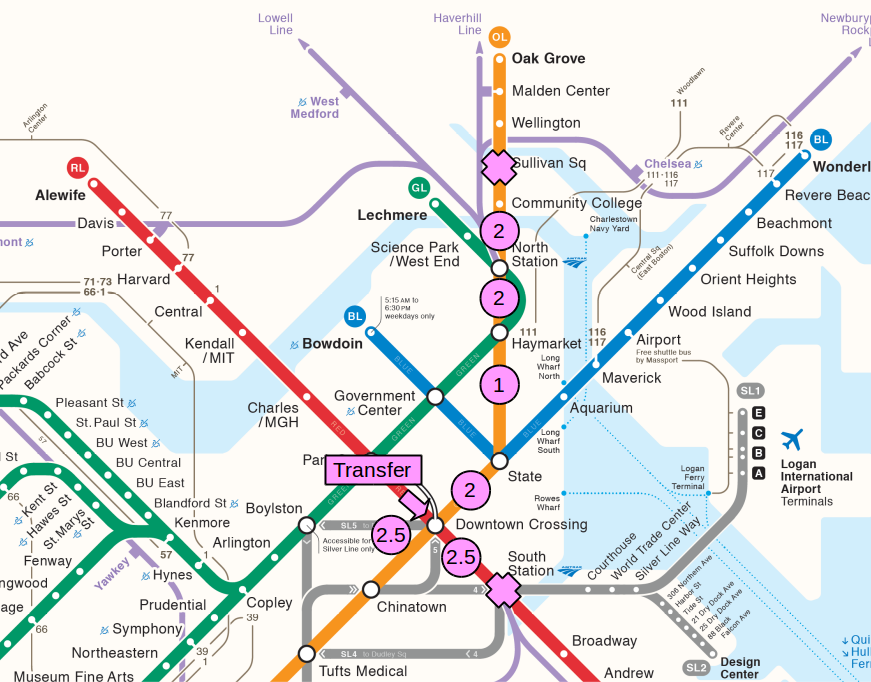
\includegraphics[scale=0.8]{transfer_demonstration}\end{center}\caption{Illustration of travel time calculation for Sullivan Square to South Station, in Boston.}\label{fig:f2}
\end{figure}



\subsection{Regression Analysis}

Regression models for station level ridership have used ordinary least squares regression\cite{Kuby2004, Taylor2008, Currie2011, Durning2015, Gutierrez2011} to generate predictions. We will investigate the applicability of more complex regression models 






 
\bibliographystyle{unsrt}
\pagebreak\bibliography{bibrefs}





\end{document}